\documentclass[
 reprint,
%preprint,
%preprintnumbers,
 amsmath,amssymb,
 aps,
%pra,
prb,
%rmp,
% prstab,
%prstper,
floatfix
]{revtex4-2}

\usepackage{lipsum}
\usepackage{graphicx}
\usepackage{dcolumn}
\usepackage{bm}
\usepackage{hyperref}
\usepackage{enumitem}

\begin{document}

\preprint{APS/123-QED}

\title{Comparing Olympic Host Cities' Availability of Entertain and Dining Venues}

\author{John Truong}
\affiliation{%
 University at Buffalo\\
 jtruong@buffalo.edu
}

\date{\today}

\begin{abstract}
    The International Olympic Committee selects host cities based on a number fo criteria. We explore correlations between host cities to find if there are other factors that determine if a city is capable of hosting the international event. In particular, we look at whether the prevalence of entertainment and dining venues for visiotrs plays any role at all. We determine that while there is a positive correlation between the number of venues and hosting the Olympics, having fewer venues relative to other cimilar cities does not prevent a city from hosting, quite possibly due to other determining factors which are not explored in this work.
\end{abstract}

\maketitle

\section{Introduction}
    For a city to be chosen to host the Olympics, they go through a vigorous vetting process by the International Olympic Committee (IOC). The primary qualifications that each city must have just to get past the first round of the selection process include~\cite{chepkemoi_how_2018}:
    \begin{enumerate}
        \item Ample lodging and accomodations for visitors
        \item An efficient transportation infrastructure to move people from event to event
        \item Proper security to protect fans and athletes
    \end{enumerate}
    For this paper, we want to see if we there are certain other qualifications that make a city Olympic-worthy. You can consider them as hidden variables. While this may not be a consideration by the IOC, visitors and athletes will, without a doubt, explore the host city and see what it has to offer. For this work in particular, we'll look at dining and entertainment venues present in the city to see if there is any connection between the number of venues and whether a city can host the Olympics or not. If we do find any correlation, this could  allow potential host cities to target and develop their local businesses in areas that they may be lacking in the hopes of one day hosting the Olympics.

\section{Data Sources}
    In order to perform this analysis, we'll need to obtain a variety of data. We'll need data on cities throughout the world (both host and non-host cities), their location data and any other relevant data, and lastly, venue data for each city.
    \subsection{Cities}
    For our list of cities, we'll restrict ourselves to highly populated cities, as they are most likely be able to host large-scale international events. So for this purposes of this paper, we'll restrict ourselves to only cities with populations of over $1,000,000$ people. Luckily for us, the U.N. already provides data for cities of populations greater that $100,000$~\cite{un_pop}. We'll just have to parse through and filter out the smaller cities.

    Table 8 in the UN Yearbook contains an Excel sheet with the population data for all cities with populations above $100,000$ and all capital cities regardless of population. The challenge with processing this dataset is primarily in the formatting so it needs to be cleaned first.

    The main source of headache is that the data is not a standard but rather an Excel formatted sheet. The first column of the data is a hierarchal structure with each tier as follows:
    \begin{enumerate}[topsep=0pt,itemsep=-1ex,partopsep=1ex,parsep=1ex]
        \item Continent
        \item Country
        \item Source of Data
        \item City
    \end{enumerate}
    where each tier is indented by that amount. These indents are not tab characters that can be processed if exported as a csv file but rather a formatting object with Excel. These need to be processed with VBA which we have done. After the Excel file was cleaned up, we went through and manually fixed any formatting errors, renamed some cities to their more common names or English names (i.e. Republic of Korea to South Korea), etc. Lastly, it was exported to a csv file that Python can handle easily. The result is a file with table structure shown in table~\ref{table_unpop}..
    \begin{table}[htb]
        \centering
        \begin{tabular}{l|cc|rr}
                & Level & Capital & City Proper & Urban Area \\
                \hline\hline
        Algeria   & 0     &         &             &                      \\
        Adrar     & 1     & 0       & 200834      & 0                    \\
        Algiers  & 1      & 1        & 2712944    & 0                      \\
                \vdots & \vdots & \vdots & \vdots & \vdots
        \end{tabular}
        \caption{Example output after processing the UN population data within Excel. The `Level' column indicates whether that row is a country (0) or a city (1). All cities belong to the country above them. The `Capital' column indicates whether the city is national capital or not. The remaining two columns are the population data given. Some countries share their population data strictly within city limits while others use describe a greater metropolitan area.}
        \label{table_unpop}
    \end{table}
    \begin{table*}[tb]
        \centering
        \begin{tabular}{ll|cr|ccr|rr}
        Country & City & Capital & Population & Winter & Summer & Year & Latitude & Longitude \\
        \hline\hline
        Algeria&Algiers&1&2712944&0&0&0&36.7753&3.0601\\
        Andorra&Andorra La Vella&1&22205&1&0&2010&42.5069&1.5212\\
        China&Beijing&1&18796000&2&2&2022&39.9062&116.3912\\
        Italy&Milano&0&1358871&2&1&2026&45.4668&9.1905\\
        South Korea&Pyeongchang&0&0&2&0&2018&37.3705&128.3903
        \end{tabular}
        \caption{Example table of our city data with some select cities shown. Note that Pyeongchang has hosted the Winter Olympics but is not a city nor did it have population above $100,000$ so it did not appear in the UN dataset.}
        \label{table_locData}
    \end{table*}
    Further processing in done using Pandas in Python. The two population columns were merged by taking the higher of the two values. `Country' and `City' columns were formed along with keeping the `Capital' column. Something important to note is that population data for Chinese cities outside of Beijing were not present in the dataset.

    We can then cross reference this with the list of past and future cities who've placed bids to host the event~\cite{wiki_hosts} to get our set of cities. In particular we used the tables ``All-time Summer (Winter) Olympics bids'' saving the country, city, whether they hosted or simply bid, and the most recent year they placed a bid. Keep in mind for host cities that the most recent year they bid may not necessarily be the most recent year they hosted.

    Cities were assigned a value of $2$ if they were selected to be hosts at any point in time while those who made it to the final stage but weren't ever selected were assigned a value of $1$. When we ultimately merge this data with the population data, cities they have never bidded will be given a default value of $0$. We can define a ``worthiness'' score for each city by summing these two values.
    \begin{equation*}
        \textrm{Worthiness} = \textrm{Summer} + \textrm{Winter}
    \end{equation*}
    Thus, the worthiness score has a maximum value of $4$ (similar to a GPA), which only Beijing has.

    % City data
    \subsection{Geolocation/Mapping}
    Once the list of cities is obtained, we'll also need the location data for each city for both mapping purposes and to eventually get venue data from Foursquare. For this, we'll simply use the \emph{geopy} library in Python along with a geocoder like Nominatim. Nominatim has a limit of $1$ request per second so as long as our list of cities isn't too long, this should be a quick process. The cities are shown on figure~\ref{map} and our final table of data is shown in table~\ref{table_locData}.

    \begin{figure*}[htb]
        \centering
        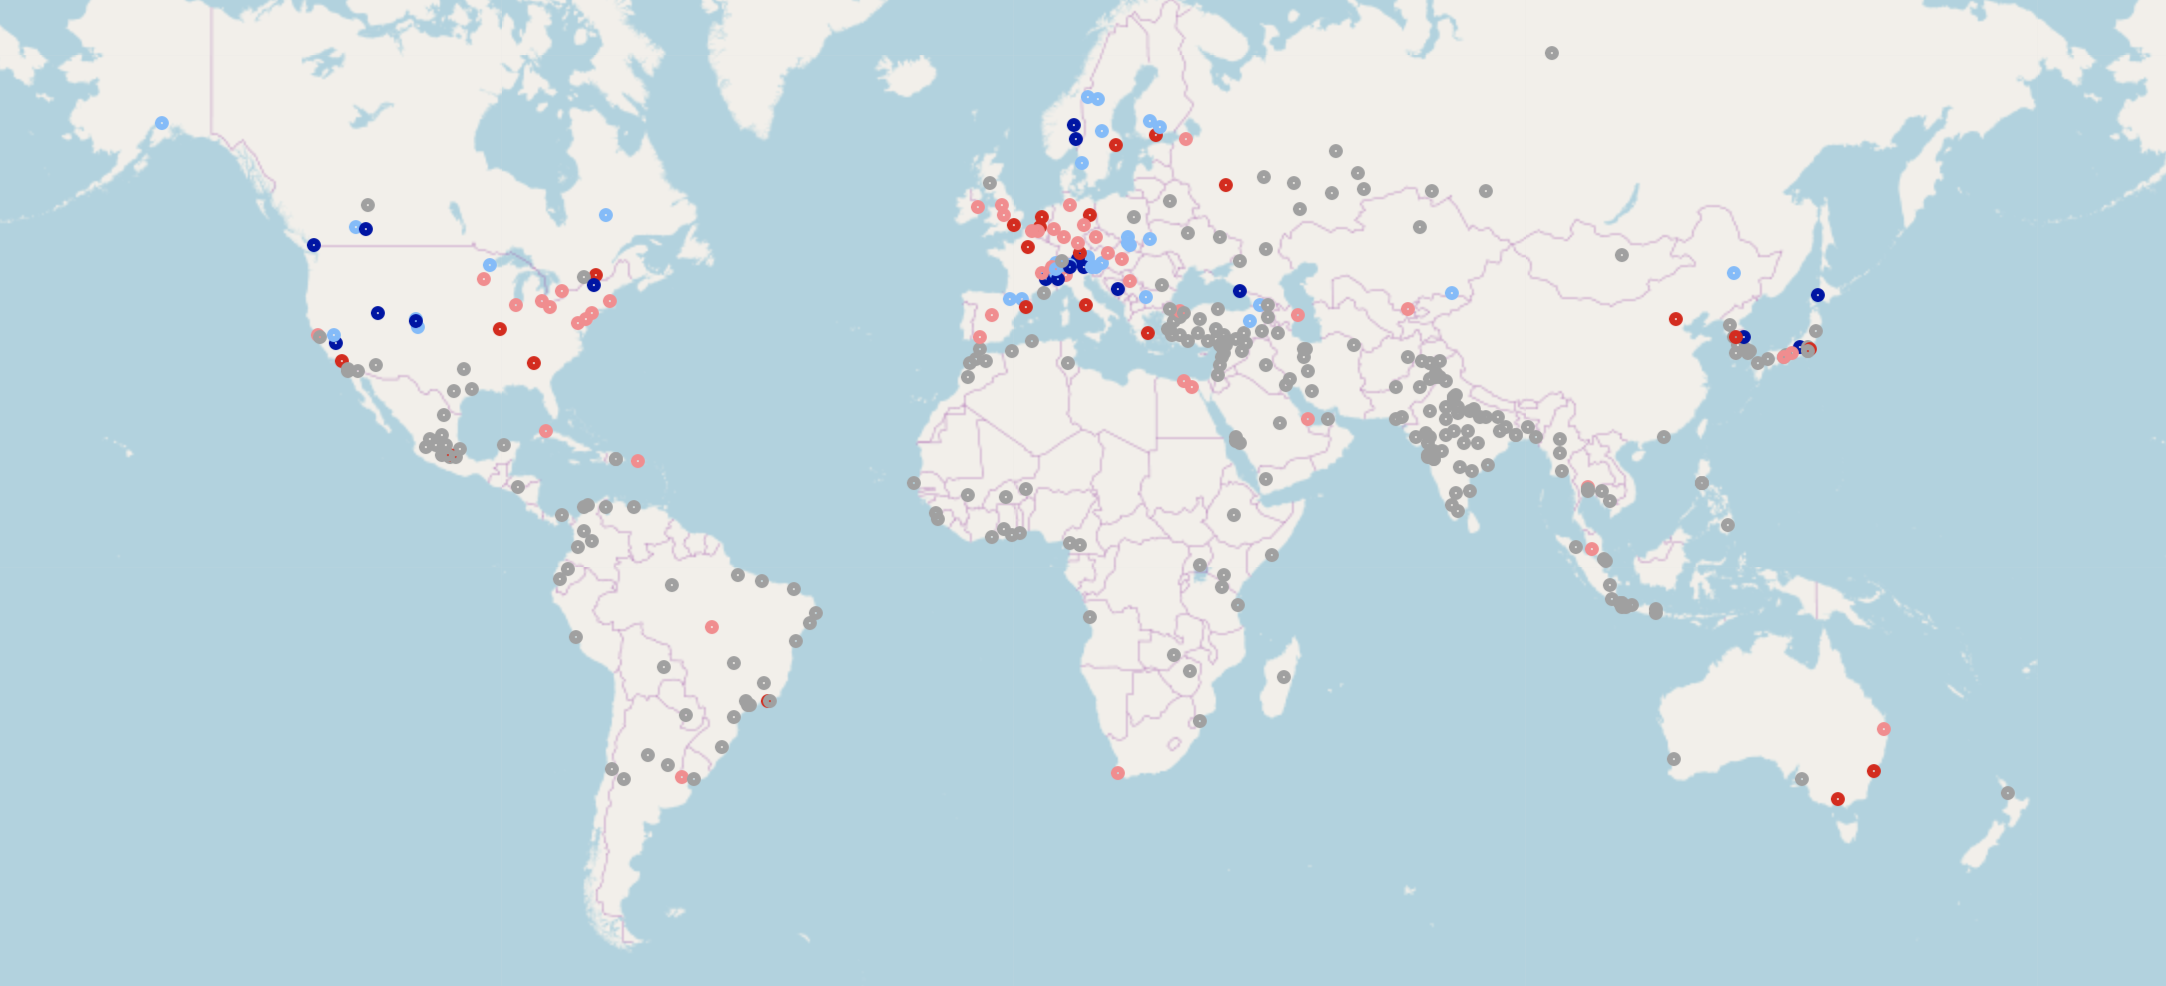
\includegraphics[width=\textwidth]{../figures/world_map.png}
        \caption{Cities with populations $>1,000,000$. Cities marked red (blue) are those that have hosted the Summer (Winter) Olympics while the lighter shades are those that have bid but were not selected. For cities that have bid/hosted both seasons, priority was given to the Summer Olympics and are colored red. Gray cities have never bid for the Olympics.}
        \label{map}
    \end{figure*}

    % Foursquare data
    \subsection{Venues}
    We'll be using the Foursquare Places API~\cite{foursquare} to obtain the venue data. The API allows us to filter by venue category which is great since we are only interested in dining and entertainment, so we can selectively search for those particular venues, with the goal being to simply get a count of all venues. We don't need specific data pertaining each individual venue at for this analysis, just the category. Collecting venue data provided somewhat of a challenge since Foursquare has a limit of $50$ results returned per call. Fortunately, their Explore endpoint has an offest setting allowing for pagination. Thus we just repeated called the API while increasing the offset of each call by $50$. We stopped once Foursquare returned zero new results within a radius of $30$ kilometers. We also restricted our search by category, so we ended up searching each city four times, once for each category of interest:
    \begin{enumerate}[topsep=0pt,itemsep=-1ex,partopsep=1ex,parsep=1ex]
        \item Arts and Entertainment
        \item Food
        \item Nightlife
        \item Outdoors and Recreation
    \end{enumerate}
    This search was repeated for each city in our list, the consolidated by counting the number of venues returned. The final venue counts were then merged with the location data table to give us our final data to analyze, given in table~\ref{table_final}.
    \begin{table}[htb]
        \centering
        \begin{tabular}{ll|c|rrrr}
        Country & City & \ldots & A\&E & Food & Nightlife & O\&R \\
        \hline\hline
        Algeria&Algiers& & 8 & 51 & 8 & 31 \\
        Andorra&Andorra La Vella&& 12 & 158 & 48 & 101\\
        China&Beijing& \ldots& 129 & 133 & 112 & 139 \\
        Italy&Milano& & 132 & 238 & 224 & 232 \\
        South Korea&Pyeongchang& & 5 & 52 & 5 & 33
        \end{tabular}
        \caption{Venue counts for each category}
        \label{table_final}
    \end{table}

    With this final set of data, we hope to find some sort of correlation between the number of venues in any given city and whether is has bid for or hosted the Olympics before.

\section{Methodology}
    A quick glance at the raw data reveals some interesting correlations (Figure~\ref{raw_corr}). We see that the Winter Olympics are more dependent on the city's latitude that the Summer Olympics. This result should be pretty obvious due to the need for colder weather during the Winter Olympics. What is more interesting is that the Winter Olympics don't show as strong a correlation to venue counts as the Summer Olympics. Seems like the Summer games depend on cities having more things to do for the guests. These exploratory results though are skewed pretty heavily by more populated cities, so for the actual analysis we'll be looking at the data per capita.
    \begin{figure}[htb]
        \centering
        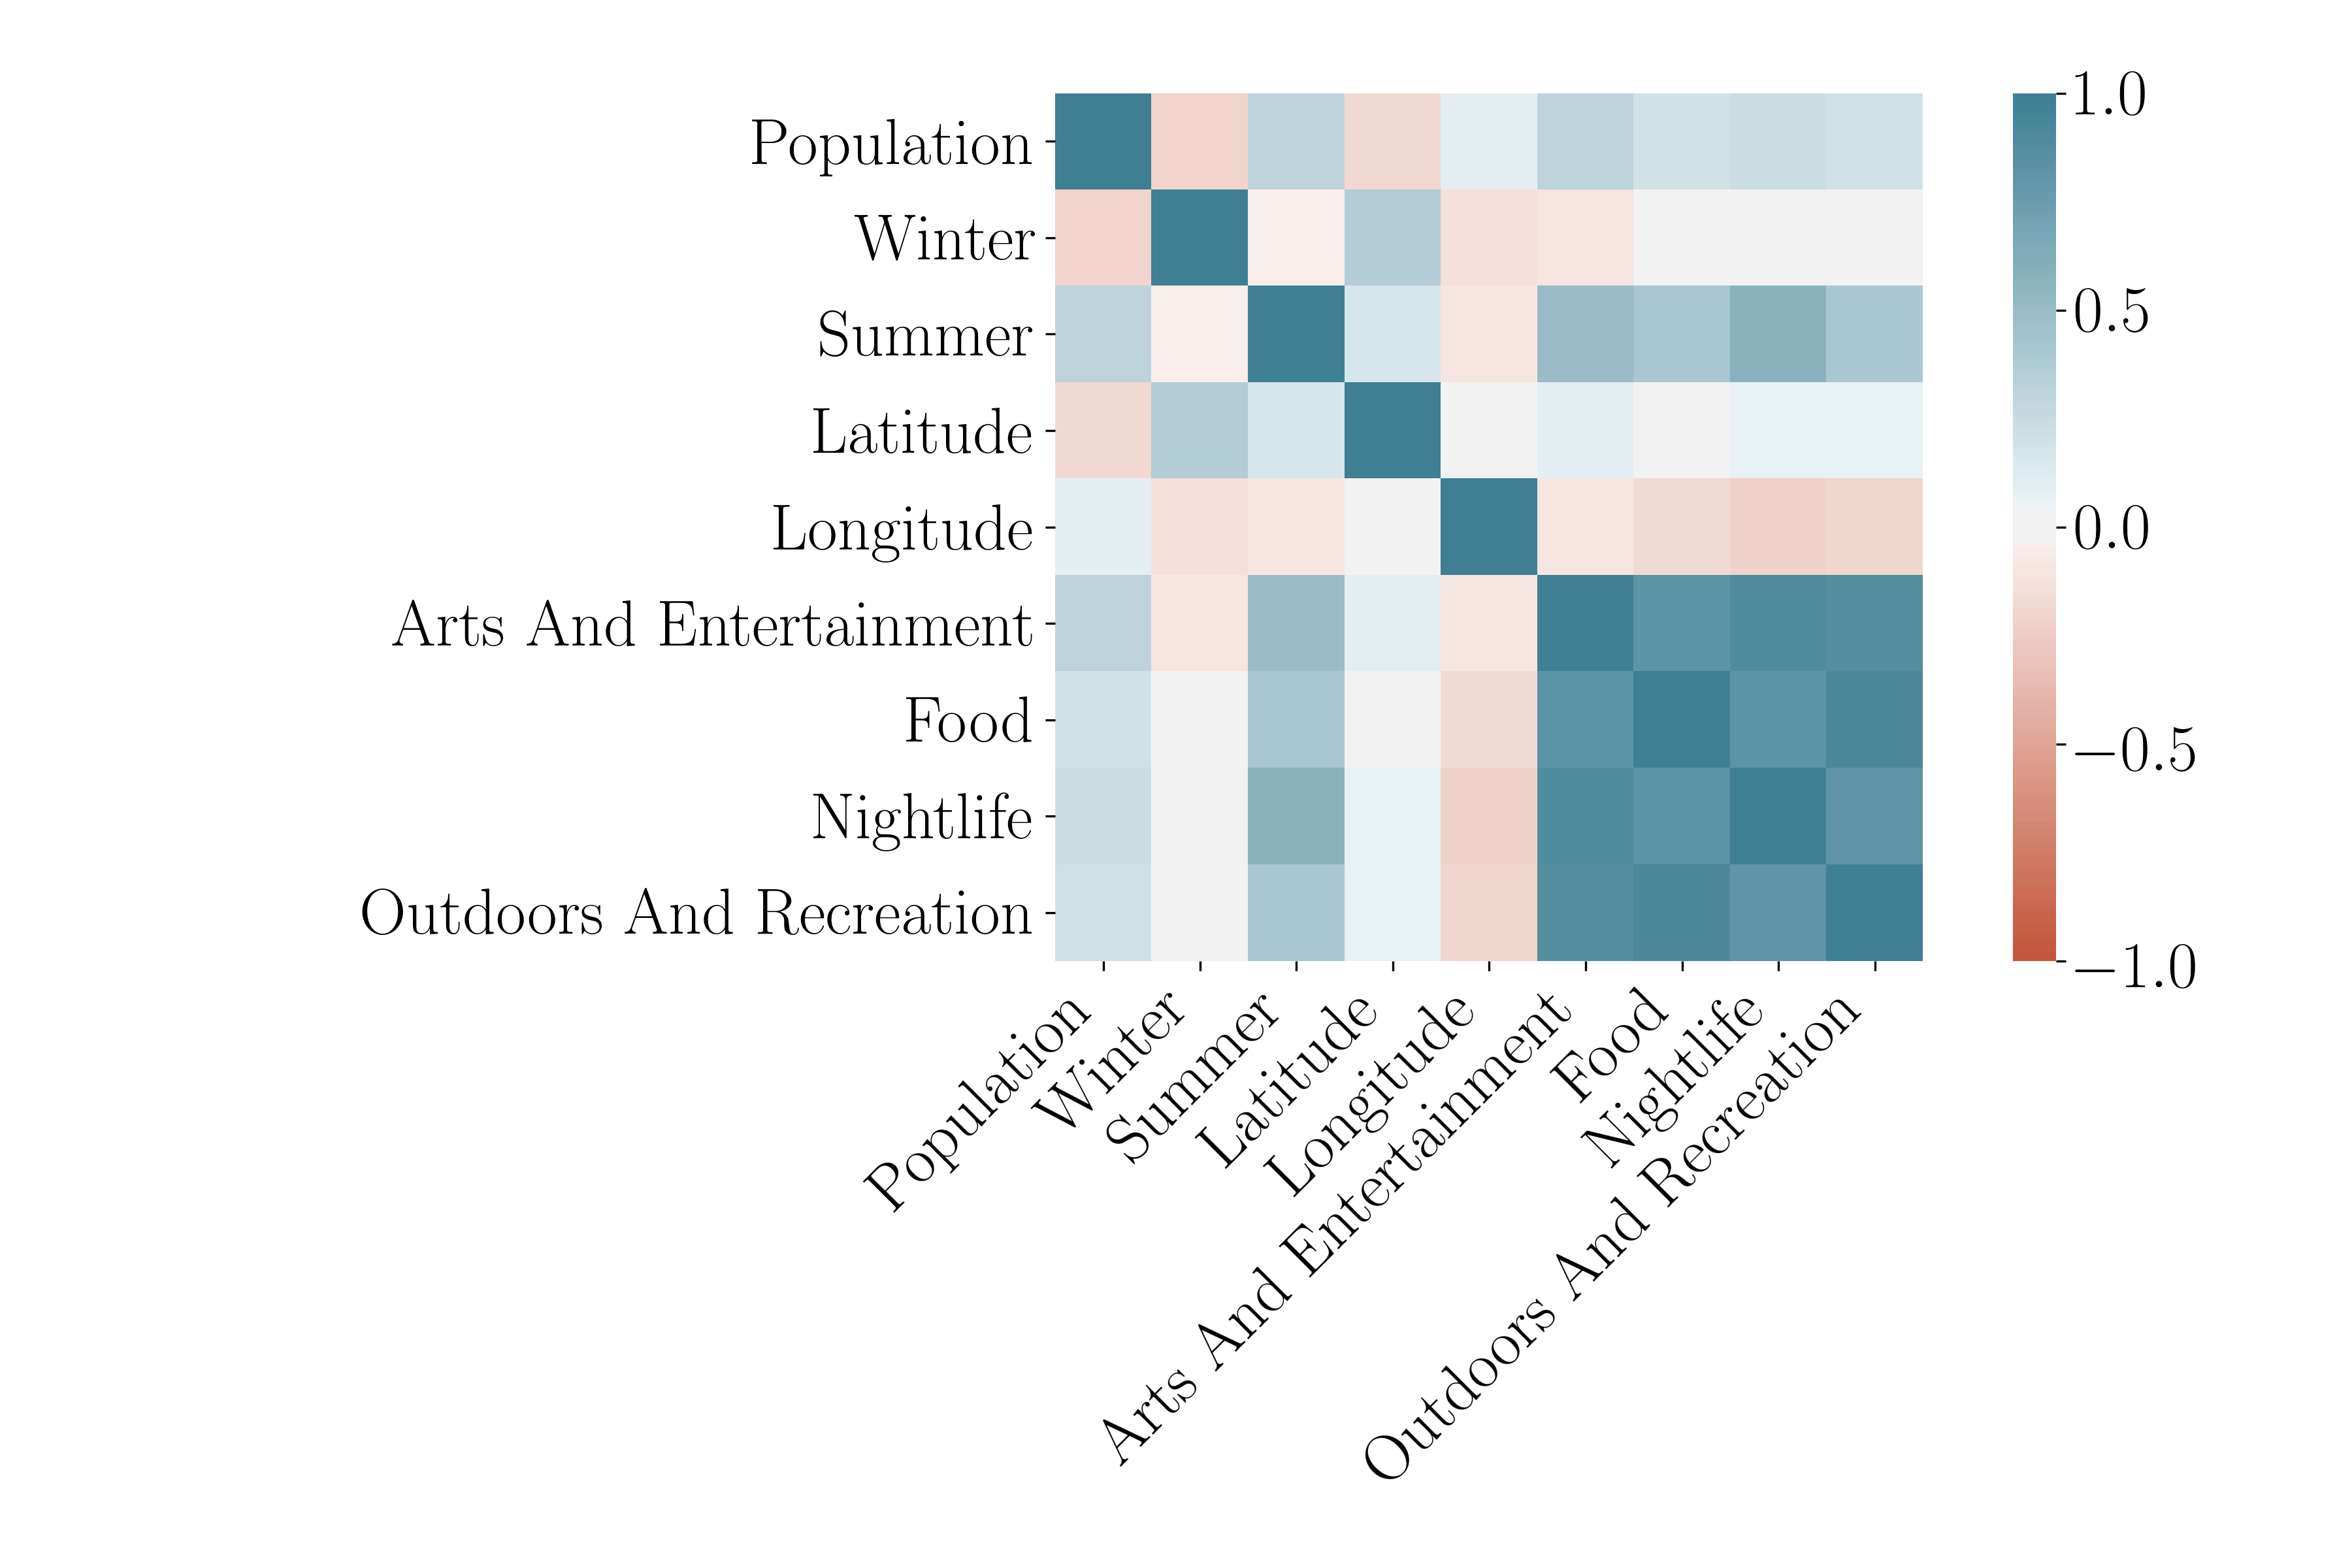
\includegraphics[width=\columnwidth]{../figures/correlation.png}
        \caption{Correlation matrix for the raw data. We see stronger correlation between the Summer Olympics and the venue counts. There is also a stronger correlation for the population too. This indicates that the possibility that the correlation is actually between the population and the venue count, which is sensible. To remove this possibility, we use per capita data instead.}
        \label{raw_corr}
    \end{figure}
    \begin{figure}[htb]
        \centering
        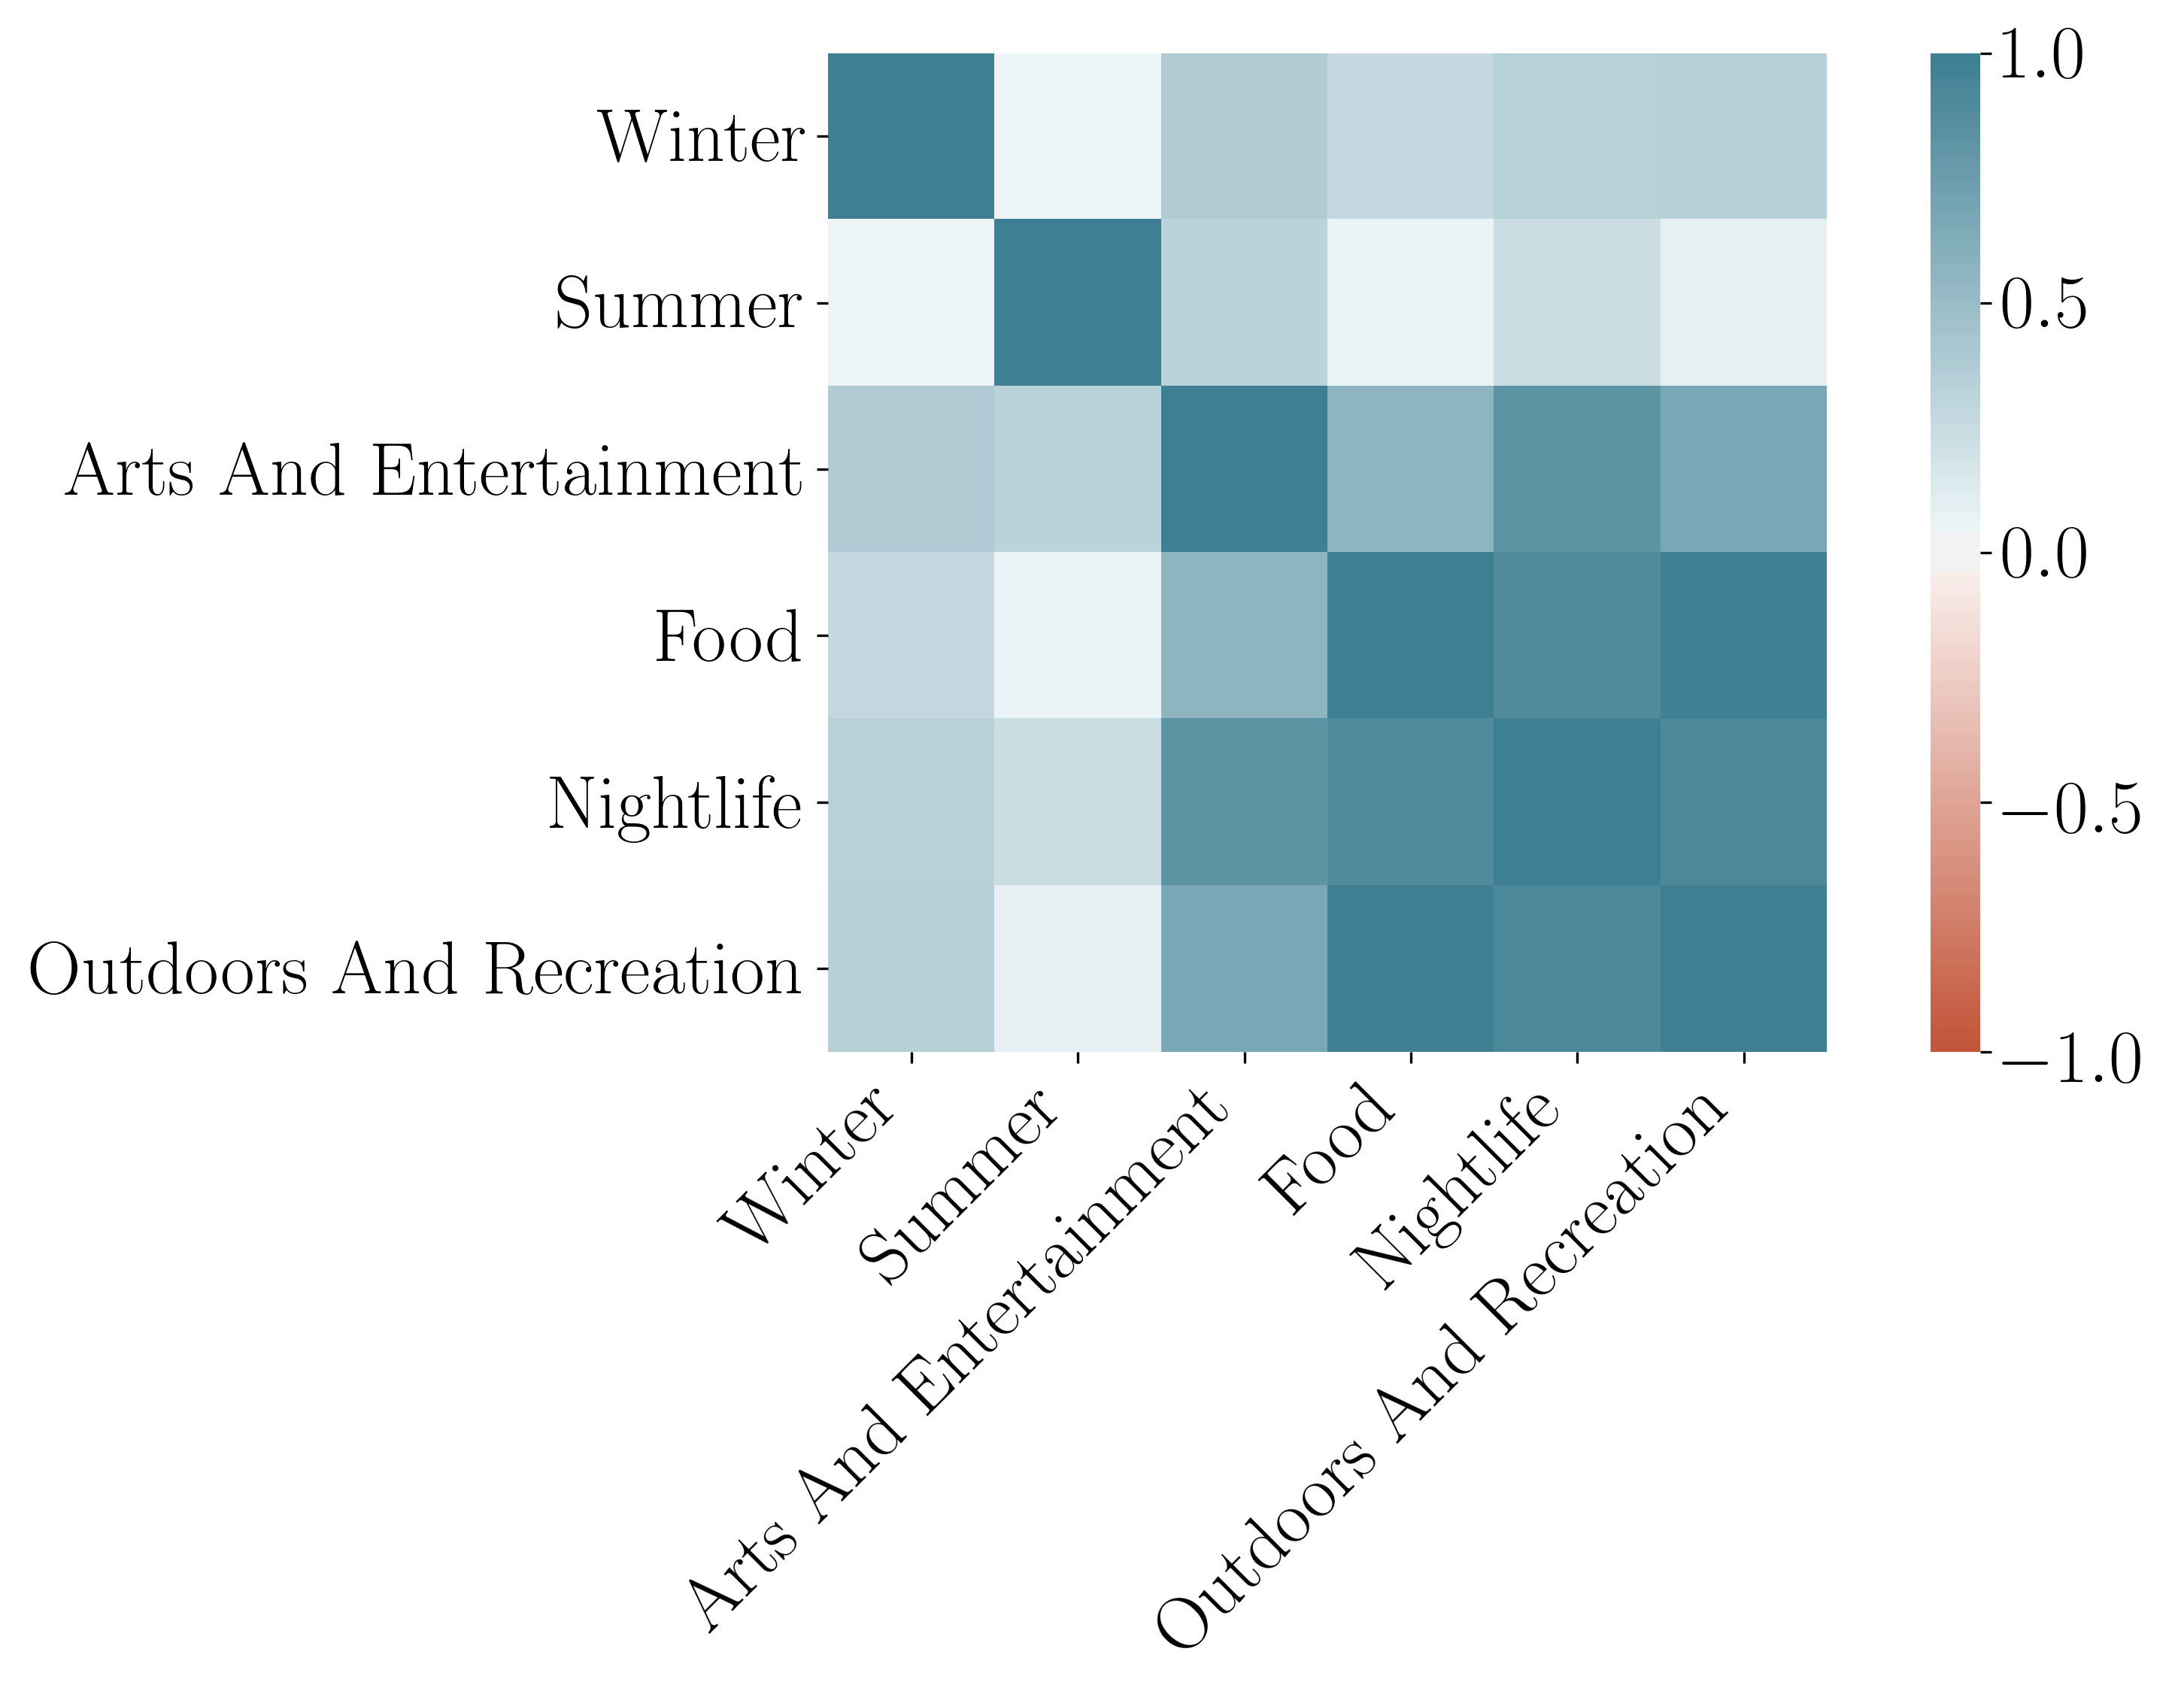
\includegraphics[width=\columnwidth]{../figures/correlation_percapita.png}
        \caption{Correlation matrix for the per capita data. Now both Winter and Summer games have a positive correlation with the venue data. We also see that the Winter Olympics has a stronger correlation to the number of outdoor activities than the Summer Olympics.}
        \label{corr_percapita}
    \end{figure}
    We can also visualize the data by using scatter plots of any two of the four categories for the two axes, as shown in Figures~\ref{avd_scatter} and~\ref{nvd_scatter}.
    \begin{figure}[htb]
        \centering
        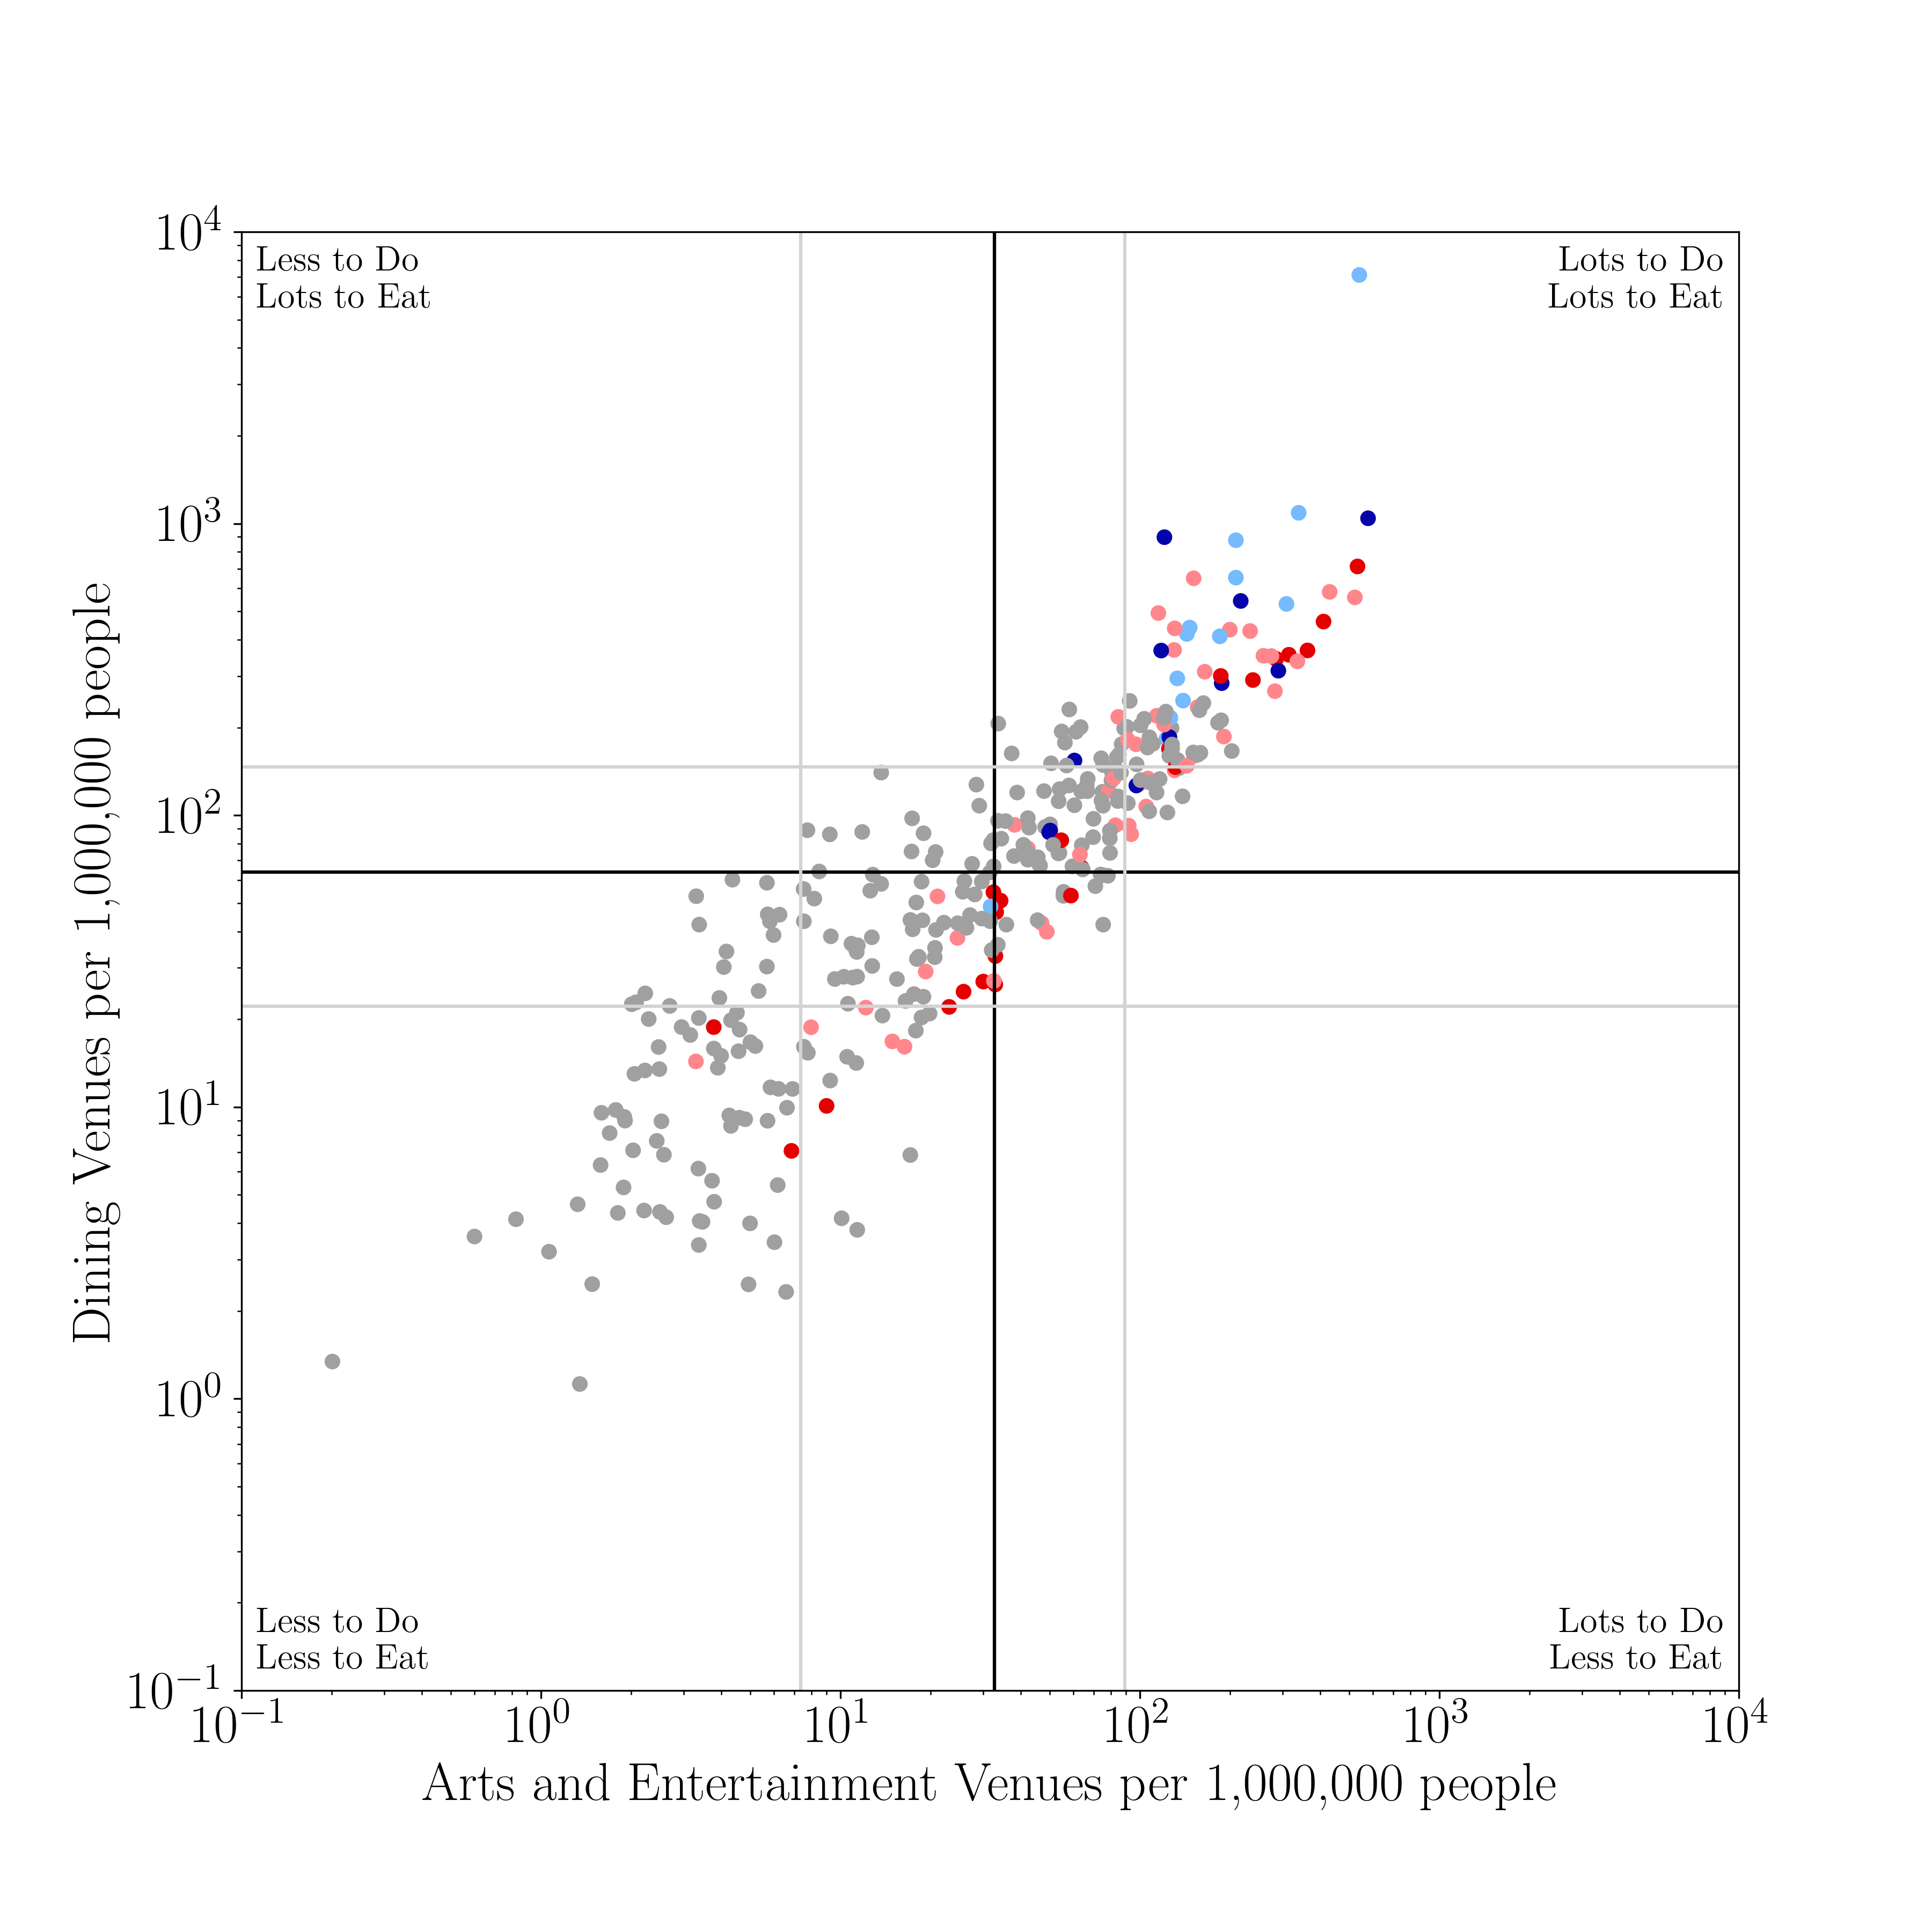
\includegraphics[width=\columnwidth]{../figures/foodandentertainment_percapita.png}
        \caption{Scatter plot for Arts and Entertainment venues and Dining venues. Colors are as defined in Figure~\ref{map}. We see that Olympic hosts tend to be in the upper-right corner where their venues per capita are above the 75th percentile. The one noticable outlier point is the city of Andorra La Vella.}
        \label{avd_scatter}
    \end{figure}
    \begin{figure}[htb]
        \centering
        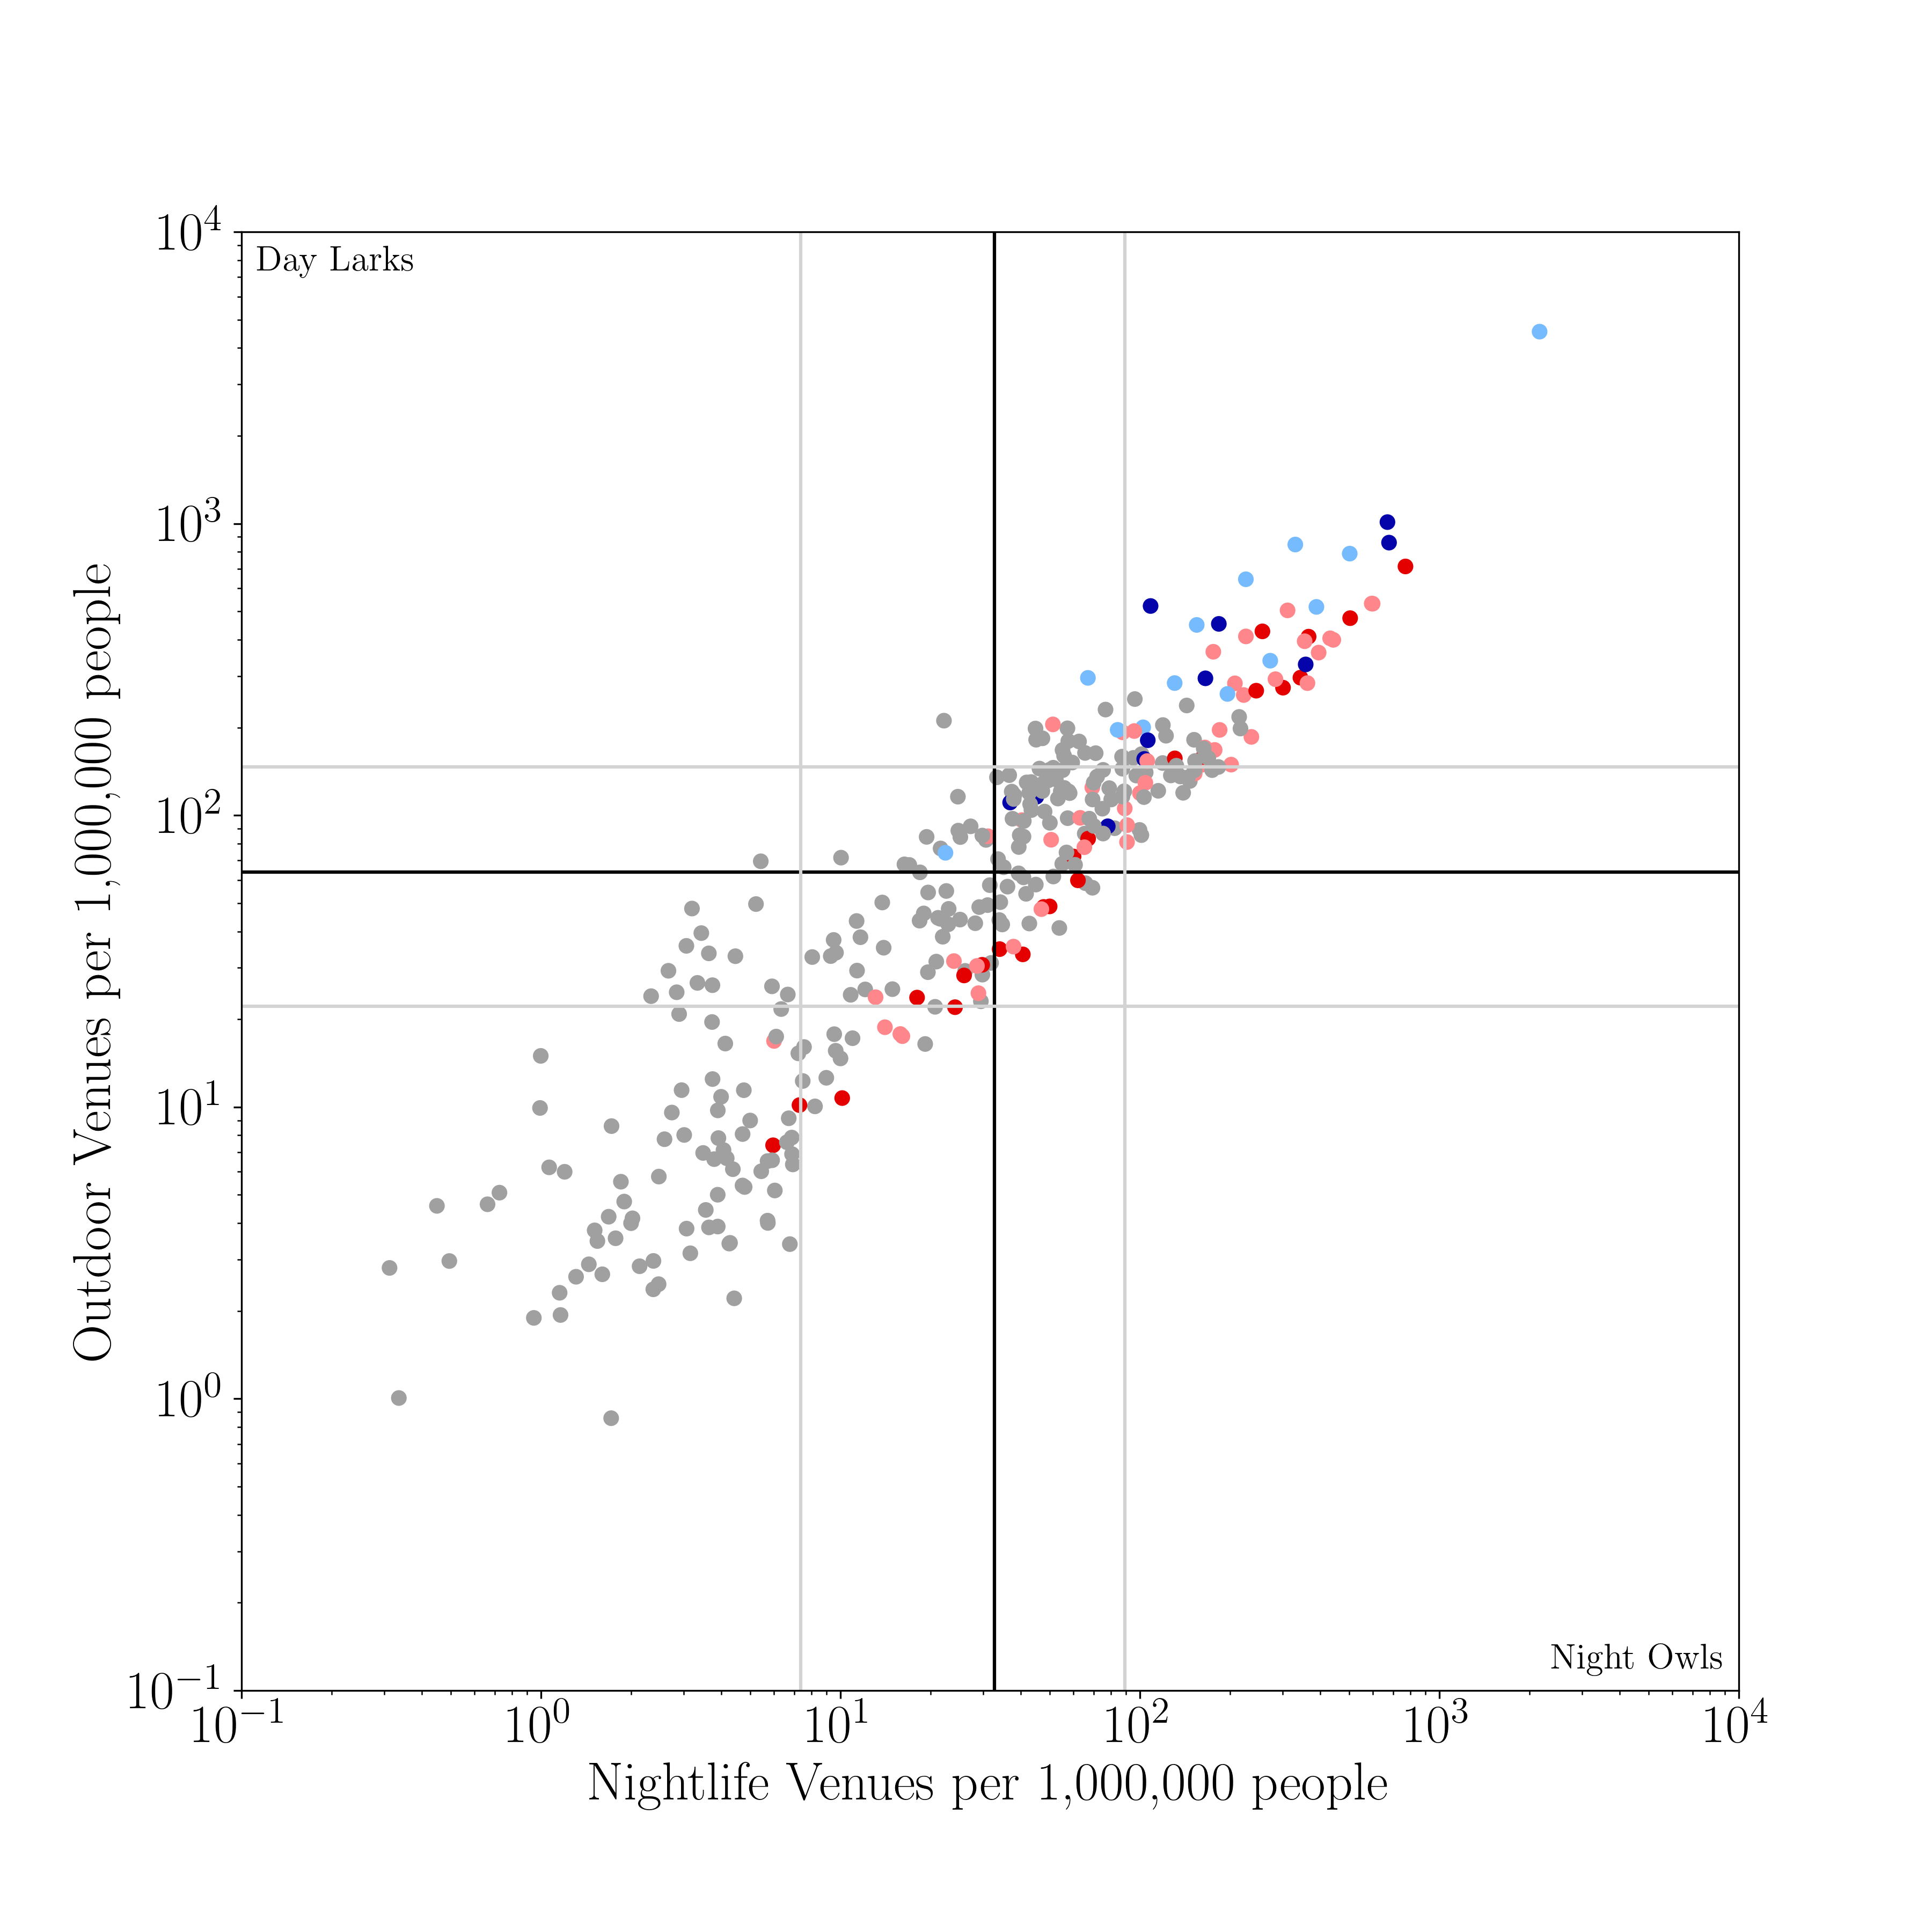
\includegraphics[width=\columnwidth]{../figures/nightanddaylife_percapita.png}
        \caption{Scatter plot for Nightlife venues and Outdoor venues. IN addition to the same conclusion as in Figure~\ref{avd_scatter}, we can also see that Winter cities tend to have more Outdoors and Recreation venues than Summer cities that have the same amount of Nightlife venues. This is consistent with what we saw in the correlation heat map, Figure~\ref{corr_percapita}.}
        \label{nvd_scatter}
    \end{figure}
    These scatter plots reveal that per capita venue counts are indeed a hidden variable for Olympic ``worthiness''.

    We next try to classify cities by their worthiness. For this step, we use a k-means algorithm to segregate the cities using all four categories. We decided to use clusters. Table~\ref{cluster_table} shows some select cities in each cluster\footnote{Note: The cluster numbers used in this paper have been reordered from the ones returned by the clustering algorithm for clarity.}.
    \begin{table}
        \centering
        \begin{tabular}{r|l}
            Cluster & City \\
            \hline\hline
            0 & Sydney, Australia \\
              & Islamabad, Pakistan \\
              & Beijing, China \\
              & Los Angeles, California, USA \\
              & Paris, France \\
              & Tokyo, Japan \\
              & \vdots \\
            \hline
            1 & Chicago, IL, USA \\
              & Sapporo, Japan \\
              & Milan, Italy \\
              & Berm, Switzerland \\
              & \vdots \\
            \hline
            2 & Antwerp, Belgium \\
              & Denver, CO, USA \\
              & Sochi, Russia \\
              & \vdots \\
            \hline
            3 & Andorra la Vella, Andorra
        \end{tabular}
        \caption{Sample of some cities in each cluster sorted by their average number of venues per capita. Cluster 3 is only Andorra la Vella and no others.}
        \label{cluster_table}
    \end{table}

\section{Results}
    Using our simple metric for Olympic worthiness, we compute the average worthiness for each cluster, summarized in Table~\ref{summary}. What is shown is that as the Olympic worthiness of a cluster goes up, the size of that cluster goes down (with the exception of Andorra), which is consistent with what one would expect.
    \begin{table}[h!]
        \centering
        \begin{tabular}{r|ccc}
            Cluster & Cities & Host Cities & Average Worthiness \\
            \hline\hline
            0 & 225 & 16 & 0.22 \\
            1 & 100 & 9  & 0.46 \\
            2 & 26  & 10 & 1.46 \\
            3 & 1   & 0  & 1.00
        \end{tabular}
        \caption{Summary of each cluster.}
        \label{summary}
    \end{table}

\section{Discussion}
    What is quite interesting are which cities are in each cluster. The least worthy cluster, according to this work, contains Tokyo, Beijing, Paris, and LA. These are 4 of the next 5 host cities. Milan is the only one not in that cluster, but it is in the second least worthy cluster.

    What this does tell us is that if a city wanted to host the Olympics, it is most definitely beneficial to have more things for guests to do while in town. But it also doesn't necessarily eliminate them from contention if they don't have as many venues as seen in the cities set to host for the next 10 years.

\section{Conclusion}
    In the end, we did find that the number of venues per capita is indeed a hidden variable in determining whether a city is fit to host the Olympics or not. But our work also shows that there are potentially more variables that we haven't explored yet, such as average temperature.

    In this work, we used a simple clustering method to classify cities. In the future, we would like to implement a supervised machine learning algorithm to classify cities instead. This would allow us to computationally predict the probability of a city outside of our dataset hosting the Olympics. This could potentially require a larger training dataset, more than the $300$ cities we have now.

\bibliography{report}

\end{document}

